% \section{Training Protocol}
% In this section we provide a description of the algorithm and training protocol.

\section{Training details}
\subsection{Training Hyperparameter Settings}
The agent interacts with the environment via episodes of fix length $T = 500$ steps. The algorithm has access to the dataset $\mathcal{M}$ containing observation-only motions. Similarly to~\citep{TirinzoniTFGKXL25zeroshot}, the initial state distribution of an episode is a mixture between randomly generated falling positions and states in $\mathcal{M}$ (motion initialization). We use prioritization to sample motions from $\mathcal{M}$ and, inside a motion, the state is uniformly sampled. We use an exponential prioritization scheme based on the agent's ability to track a motion. To have a more fine-grained prioritization, we split the $40$ LAFAN1~\citep{HarveyYNP20lafan1} motions into chunks of $10$ seconds. 
Every $N_{\mathrm{eval}}$ interaction steps, we evaluate all the motions and update the priorities base on the earth mover’s distance~\citep[EMD]{RubnerTG00}. For each motion $m \in \mathcal{M}$, the priority is given by
\[
p(m) \propto 2^{\max\Big\{0.5;\;\min\big\{\mathrm{EMD}(m), 2\big\}\Big\} \cdot 4}
\]

We take inspiration from the recipe in FastTD3~\citep{Seo2025fasttd3} to scale up unsupervised off-policy RL to using massively parallel environments. We use standard MLPs for all the components of the model, even for handling history. We simulate $N_{\mathrm{env}}$ parallel (and independent) environments at each step. We scale the buffer size accordingly to the number of environments, following the rule $N_{\mathrm{buffer}} \times N_{\mathrm{env}} \times T$. We use a batch size of $N_{\mathrm{batch}}$ and we use an update-to-data ratio of $N_{\mathrm{ups}}$ gradient steps per (parallel) environment step. We train the model for a total number of environment steps $N_{\mathrm{train}} = \frac{N_{\mathrm{grad}}N_{\mathrm{env}}}{N_{\mathrm{ups}}}$. We report the value of these parameters in Tab.~\ref{tab:params}, the missing parameters are as in~\citep{TirinzoniTFGKXL25zeroshot}.

% \begin{figure}[h]
% \begin{minipage}[t]{.48\textwidth}
\begin{table}[h]
    \centering
    \footnotesize % 缩小字体
    \begin{tabular}{lc}
    \toprule
    \textbf{Parameter} & \textbf{Value} \\
    \midrule
    \multicolumn{2}{l}{\textbf{Environment and Training Setup}} \\
    \midrule
    History Length $H$                  & 4 \\
    Episode Length $T$                  & 500 \\
    $N_{\mathrm{env}}$                  & 1024 \\
    $N_{\mathrm{batch}}$                & 1024 \\
    $N_{\mathrm{ups}}$                  & 16 \\
    $N_{\mathrm{grad}}$                 & 3M \\
    $N_{\mathrm{train}}$                & $\approx 192$M \\
    $N_{\mathrm{buffer}}$               & 10 \\
    $N_{\mathrm{eval}}$                 & $N_{\mathrm{train}}/20$ \\
    Buffer Size (transitions)           & $\approx 5$M \\
    Discount Factor                     & 0.98 \\
    Number of Seeding Steps             & $10 \cdot N_{\mathrm{env}}$ \\
    Fall Initialization Probability     & 0.3 \\
    \midrule
    \multicolumn{2}{l}{\textbf{Learning and Regularization}} \\
    \midrule
    Sequence Length (Trajectory Sampling) & 8 \\
    Latent Dimension $d$                 & 256 \\
    Discriminator Reg. Coef. $\alpha_D$  & 0.05 \\
    Reward Reg. Coef. $\alpha_R$         & 0.02 \\
    Gradient Penalty                     & 10 \\
    Learning Rate $F$                    & $3 \cdot 10^{-4}$ \\
    Learning Rate $B$                    & $10^{-5}$ \\
    Learning Rate $D$                    & $10^{-5}$ \\
    Learning Rate Actor $\pi$            & $3 \cdot 10^{-4}$ \\
    Learning Rate $Q_D$                  & $3 \cdot 10^{-4}$ \\
    Learning Rate $Q_R$                  & $3 \cdot 10^{-4}$ \\
    Orthonormality Loss Coefficient      & 100 \\
    \midrule
    \multicolumn{2}{l}{\textbf{Inference}} \\
    \midrule
    Number of samples for reward inference      & 400000 \\
    Tracking look ahead in sim & Seq. length\\
    Tracking look ahead in real& 3 (real)\\
    \bottomrule
    \end{tabular}
    \caption{Training settings.}
    \label{tab:params}
\end{table}
% \end{minipage}
% \end{figure}

% \end{wraptable}

\subsection{Network Architectures}
We use a residual architecture for the actor and the critics with blocks akin to those of transformer architectures~\citep{VaswaniSPUJGKP17}, involving residual connections, layer
normalization, and Mish activation functions~\citep{Misra20}. We use an ensemble composed of two networks for critics. For discriminator and backward map we use a standard MLP with ReLu activation (see Fig.~\ref{fig:architectures}). Refer to Tab.~\ref{tab:archi} for more details.

\begin{figure}[h]
    \begin{minipage}{\textwidth}
        \centering
        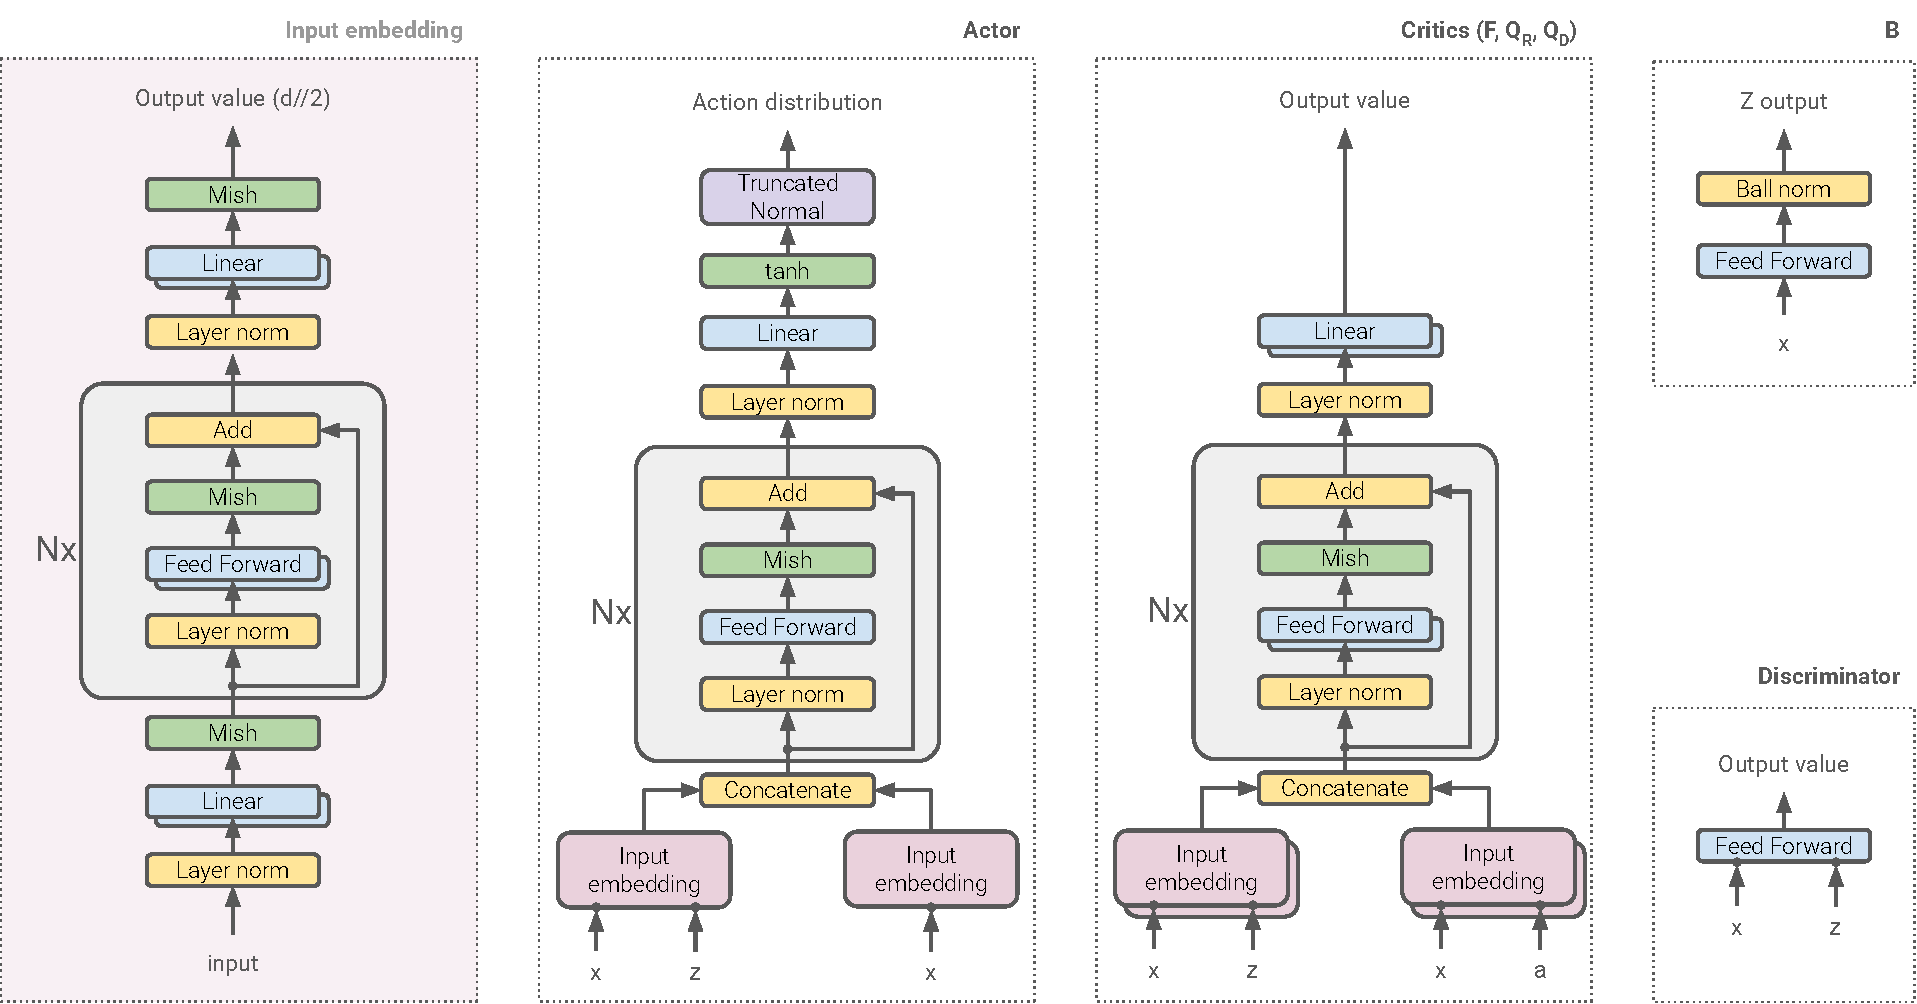
\includegraphics[width=0.9\linewidth]{image/architectures}
        \caption{Visual representation of the network architectures.}
        \label{fig:architectures}
    \end{minipage}
    % \\[.2in]
    % \begin{minipage}{\textwidth}
    %     \centering
    %     \footnotesize % 表格字体整体缩小
    %     \begin{tabular}{lcccc}
    %     \toprule
    %     \textbf{Hyperparameter} & \textbf{Critics (F, $Q_D$, $Q_R$)} & \textbf{Actor} & \textbf{Discriminator} & \textbf{B} \\
    %     \midrule
    %     Input Variables                & $(x, a, z)$ & $(x, z)$ & $(x, z)$ & $(x)$ \\
    %     Output Dim                     & F: $d$, $Q_D, Q_R$: 1 & 29 & 1 & $d$ \\
    %     Observation Variable $x$       & $(o_{t,H}, s_t)$ & $o_{t,H}$ & $(s_t, o_t)$ & $(s_t, o_t)$ \\
    %     Embedding Residual Blocks      & 4 & 4 & – & – \\
    %     Embedding Hidden Units         & 2048 & 2048 & – & – \\
    %     Residual Blocks                & 6 & 6 & – & – \\
    %     Feed Forward Hidden Layers     & 1 & 1 & 2 & 1 \\
    %     Feed Forward Hidden Units      & 2048 & 2048 & 1024 & 256 \\
    %     Activations                    & Mish & Mish & ReLU & ReLU \\
    %     Number of Parallel Networks    & 2 & 1 & 1 & 1 \\
    %     \midrule
    %     Num. Parameters (no target)    & F: 135.8M, $Q_D, Q_R$: 134.8M & 31.9M & 2.9M & 0.2M \\
    %     \midrule
    %     \textbf{Total Parameters}      & \multicolumn{4}{c}{\textbf{440.5M}} \\
    %     \bottomrule
    %     \end{tabular}
    %     \caption{Network architecture parameters used for real tests. $s_t$ is the privileged information and $o_t$ is the proprioceptive information. $o_{t,H} = \{o_{t-H}, a_{t-H}, \ldots, o_t\}$ denotes the history of proprioceptive states and actions. We exclude target networks when counting the number of parameters.}
    %     \label{tab:archi}
    % \end{minipage}
\end{figure}

\begin{table}[htbp]
    \centering
    \footnotesize
    \begin{tabular}{lcccc}
        \toprule
        \textbf{Hyperparameter} & \textbf{Critics (F, $Q_D$, $Q_R$)} & \textbf{Actor} & \textbf{Discriminator} & \textbf{B} \\
        \midrule
        Input Variables                & $(x, a, z)$ & $(x, z)$ & $(x, z)$ & $(x)$ \\
        Output Dim                     & F: $d$, $Q_D, Q_R$: 1 & 29 & 1 & $d$ \\
        Observation Variable $x$       & $(o_{t,H}, s_t)$ & $o_{t,H}$ & $(s_t, o_t)$ & $(s_t, o_t)$ \\
        Embedding Residual Blocks      & 4 & 4 & – & – \\
        Embedding Hidden Units         & 2048 & 2048 & – & – \\
        Residual Blocks                & 6 & 6 & – & – \\
        Feed Forward Hidden Layers     & 1 & 1 & 2 & 1 \\
        Feed Forward Hidden Units      & 2048 & 2048 & 1024 & 256 \\
        Activations                    & Mish & Mish & ReLU & ReLU \\
        Number of Parallel Networks    & 2 & 1 & 1 & 1 \\
        \midrule
        Num. Parameters (no target)    & F: 135.8M, $Q_D, Q_R$: 134.8M & 31.9M & 2.9M & 0.2M \\
        \midrule
        \textbf{Total Parameters}      & \multicolumn{4}{c}{\textbf{440.5M}} \\
        \bottomrule
    \end{tabular}
    \caption{Network architecture parameters used for real tests. $s_t$ is the privileged information and $o_t$ is the proprioceptive information. $o_{t,H} = \{o_{t-H}, a_{t-H}, \ldots, o_t\}$ denotes the history of proprioceptive states and actions. We exclude target networks when counting the number of parameters.}
    \label{tab:archi}
\end{table}

% \begin{figure}[t]
%     \begin{minipage}{\textwidth}
%     \centering
%     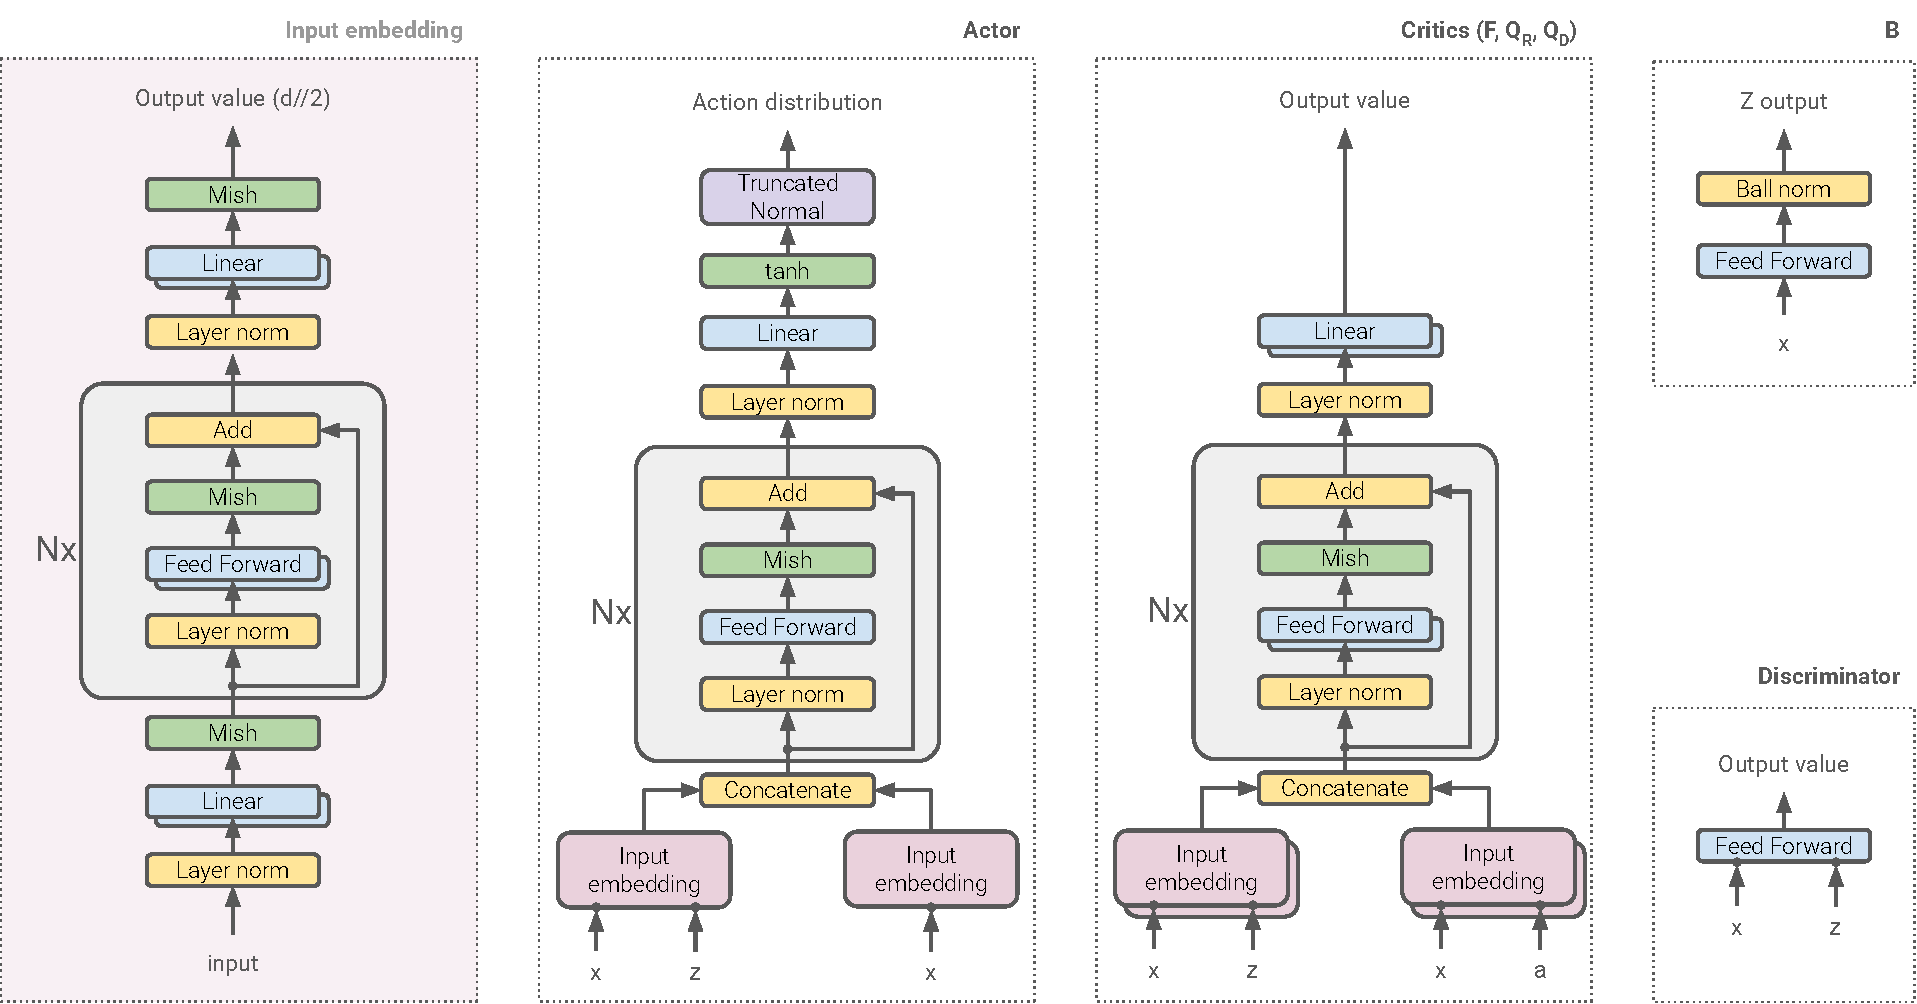
\includegraphics[width=0.99\linewidth]{image/architectures}
%     \caption{Visual representation of the network architectures.}
%     \label{fig:architectures}
%     \end{minipage}\\[.2in]
%     \begin{minipage}{\textwidth}
%     \centering
% \resizebox{.8\textwidth}{!}{%
%     \begin{tabular}{ccccc}
% \hline
% Hyperparameter & Critics (F, $Q_D$, $Q_R$)  & Actor & Discriminator & B\\
% \hline
% Input variables & $(x, a, z)$ & $(x, z)$ & $(x,z)$ & $(x)$\\
% Output dim & \makecell{F: $d$\\ $Q_D, Q_R$: 1} & 29 & 1 & $d$\\
% Observation variable $x$ & $(o_{t,H}, s_t)$ & $o_{t,H}$ & $(s_t,o_t)$ & $(s_t,o_t)$\\
% Embedding residual blocks & 4  & 4& - & -\\
% Embedding hidden units & 2048  &2048& - & -\\
% Residual blocks & 6 &  6  & - & -\\
% Feed Forward Hidden layers & 1& 1& 2 & 1\\
% Feed Forward Hidden units & 2048 & 2048 & 1024 & 256\\
% Activations & Mish &Mish& ReLu& ReLu\\
% Number of parallel networks & 2  & 1 & 1 & 1\\
% \hline
% \makecell{Number of parameters\\ (no target nets)} & \makecell{$F:135.8$M\\$Q_D, Q_R: 134.8$M} & $31.9$M & $2.9$M & $0.2$M\\
% Total number of parameters & \multicolumn{4}{c}{$846.2$M}\\
% \hline
% \end{tabular}
% }
% \caption{Network architecture parameters. We report the configuration used for real tests. Note that $s_t$ is the privileged information and $o_t$ is the proprioceptive information, $o_{t,H} = \{o_{t-H}, a_{t-H}, \ldots, o_t\}$ is the history composed by proprioceptive and action.}
% \label{tab:archi}
%     \end{minipage}
% \end{figure}


% \begin{table}[h]
% \centering
% \begin{tabular}{cccccc}
% \hline
% Hyperparameter & Critics (F, $Q_D$) & $Q_R$ & Actor & Discriminator & B\\
% \hline
% Input variables & $(x, a, z)$ &$(x, a, z)$ & $(x, z)$ & $(x,z)$ & $(x)$\\
% Output dim & F: $d$; $Q_D$: 1 & 1 & 29 & 1 & $d$\\
% Observation variable $x$ & $(h_t, s_t)$& $(h_t, s_t)$ & $h_t$ & $(s_t,o_t)$ & $(s_t,o_t)$\\
% Embedding residual blocks & 4 &  - & 4& - & -\\
% Embedding hidden units & 2048 & - &2048& - & -\\
% Residual blocks & 6 & - & 6  & - & -\\
% Feed Forward Hidden layers & 1 & 2& 1& 2 & 1\\
% Feed Forward Hidden units & 2048 & 1024 & 2048 & 1024 & 256\\
% Activations & Mish &  ReLu &Mish& ReLu& ReLu\\
% Number of parallel networks & 2 & 2 & 1 & 1 & 1\\
% \hline
% \end{tabular}
% \caption{Network architecture parameters. We report the configuration used for real tests. Note that $h_t$ is the history composed by proprioceptive and action, $s_t$ is the privileged information and $o_t$ is the proprioceptive information.}
% \label{tab:archi}
% \end{table}




\subsection{\method Algorithm Details}
We provide here a sketch of \method in (Alg.~\ref{alg:bfm.zero}). We report the algorithm without parallel networks for clarity. For clarity, we also report the FB loss here. Let $a'_i \sim \pi(x_i', z_i)$ where $x_i = (o_{i,H},s_i)$, then 
% \clearpage
\begin{equation}
\label{eq:fb.loss}
    \begin{aligned}
        \ell_{\mathrm{fb}} =&
        \frac{1}{2n(n-1)}  \sum_{i\neq k}\Big( F(x_i,a_i,z_i)^\top B(s_k',o_k')  - \gamma \overline{F}(x_i',a_i',z_i)^\top \overline{B}(s_k',o_k') \Big)^2\\
        & - \frac{1}{n} \sum_{i} F(x_i, a_i, z_i)^\top B(o'_{i}, s'_{i}) \\
        &+\frac{1}{2n(n-1)}  \sum_{i\neq k}\Big(B(s_i',o_i')^\top B(s_k',o_k')\Big)^2 - \frac{1}{n} \sum_{i\in[n]} B(s_i',o_i')^\top B(s_i',o_i')\\
        &+\frac{1}{n} \sum_{i\in[n]} \Big( F(x_i,a_i,z_i)^\top z_i - \overline{B}(s_i', o_i')\Sigma_{\overline{B}} z_i -\gamma \overline{F}(x_i',a_i',z_i)^\top z_i \Big)^2
    \end{aligned}
\end{equation}

\begin{algorithm}[h!]
	\caption{\method{} Pre-Training}\label{alg:bfm.zero}
\begin{footnotesize}
	\begin{algorithmic}[1]
    \State Initialize empty train buffer: $\mathcal{D}_{\mathrm{online}} \leftarrow \emptyset$
    \State Initialize expert buffer $\mathcal{M}$ with action-free trajectories
	\For{$t = 1, \dots$}
        \State {\scriptsize\color{YellowGreen}\textit{//Online interaction}}
        \State Sample $\boldsymbol{z}_t = \{z_e\}_{e=1}^{N_{\mathrm{env}}}\in \mathbb{R}^{N_{\mathrm{env}}\times d}$ (if needed)
        \State Execute $\boldsymbol{a}_t \sim \pi(\boldsymbol{o}_{t,H}, \boldsymbol{z}_t) \in \mathbb{R}^{N_{\mathrm{env}}\times A}$ in the \emph{simulated} environments
        \State Store $(\boldsymbol{s}_t, \boldsymbol{o}'_{t,H}, \boldsymbol{a}_t, \boldsymbol{s}_t', \boldsymbol{o}'_{t+1,H}, \boldsymbol{z}_t)$  in $\mathcal{D}_{\mathrm{online}}$

        \State {\scriptsize\color{YellowGreen}\textit{//Update}}
        \For{$j = 1, \dots, N_{\mathrm{ups}}$}
            \State Sample a batch of $n=N_{\mathrm{batch}}$ transitions $\{({o}_{i,H}, {s}_i, {a}_i, {o}_{i,H}', {s}_i', {z}_i)\}_{i=1}^{n}$ from $\mathcal{D}_{\mathrm{online}}$
            \State Sample a batch of $\frac{n}{T_{\mathrm{seq}} }$ sequences $\{(w_{j, 1}, w_{j, 2} \ldots, w_{j, T_{\mathrm{seq}}}) \}_{j=1}^{\frac{n}{T_{\mathrm{seq}} }}$ from $\mathcal{M}$ where $w = ({s}_t, {o}_t)$
            \State {\scriptsize\color{YellowGreen}\textit{//Encode expert and update discriminator}}
            \State $z_j \leftarrow \frac{1}{T_{\mathrm{seq}}} \sum_{t = 1}^{T_{\mathrm{seq}}} B(w_{j, t}) $ ; $z_j \leftarrow \sqrt{d} \frac{z_j}{\| z_j\|_2} $
            \State $\ell_{\mathrm{discriminator}} = - \frac{1}{n} \sum_{j = 1}^{\frac{n}{T_{\mathrm{seq}} }} \sum_{t = 1}^{T_{\mathrm{seq}}} \log D({w}_{j,t}, {z}_j) - \frac{1}{n} \sum_{i=1}^n \log (1-D({s}_i, {o}_i,{z}_i))$
            \State {\scriptsize\color{YellowGreen}\textit{//Update representation F and B so that } $F(s,a;z)^\top B(s') \approx M^{\pi_z}(ds'|s,a) $}
            \State Refer to Eq.~\ref{eq:fb.loss}
            \State {\scriptsize\color{YellowGreen}\textit{//note that $D$ does not use history}}
            \State Compute discriminator reward: $r_i^D \leftarrow \log (D({s}_i,{o}_i,  {z}_i)) - \log (1-D({s}_i,{o}_i,  {z}_i)), \quad \forall i \in [n]$
            \State Let $x_i = (o_{i,H}, s_i)$ and sample ${u}_i \sim \pi({o}_{i,H},{z}_i)$ for all $i\in[n]$. Then
            % \State {\scriptsize\color{YellowGreen}\textit{//Update critic $Q_D$}}
	        \State $\ell_{\texttt{critic}_D} =\frac{1}{n} \sum_{i\in[n]} \left( Q_{D}(x_i,{a}_i,{z}_i) - r_i^D - \gamma \overline{Q_D}(x_i',{a}_i,{z}_i) \right)^2$
            % \State {\scriptsize\color{YellowGreen}\textit{//Update critic $Q_R$}}
	        \State $\ell_{\texttt{critic}_R} =\frac{1}{n} \sum_{i\in[n]} \left( Q_{R}(x_i,{a}_i,{z}_i) - \sum_k r^{\mathrm{aux}}_k (x_i') - \gamma \overline{Q_R}(x_i',{a}_i,{z}_i) \right)^2$
            % \State {\scriptsize\color{YellowGreen}\textit{//Update actor }}
            \State $\ell_{\texttt{actor}} = -\frac{1}{n} \sum_{i\in[n]}\Big( F(x_i,{u}_i,{z}_i)^\top {z}_i  + \alpha_D Q_D(x_i,{u}_i,{z}_i) + \alpha_R Q_R(x_i,{u}_i,{z}_i)\Big)$
            \State {\scriptsize\color{YellowGreen}\textit{//Update target networks}}
        \EndFor
    \EndFor
	\end{algorithmic}
 \end{footnotesize}
	\end{algorithm}

\subsection{Training Environments}

To better facilitate sim-to-real transfer, we incorporated domain randomization, additive observation noise and regularization rewards in the training environment. Refer to Fig~\ref{fig:dr_and_reg} for details.

\begin{figure}[h]
\centering
\begin{tabular}{@{}c@{\hspace{2em}}c@{\hspace{2em}}c@{}}
% --- 左表：Dynamics Randomization ---
{
\footnotesize
\begin{tabular}[t]{lc}
\multicolumn{2}{c}{\textbf{Domain Randomization}} \\
\toprule
\textbf{Parameter} & \textbf{Range} \\
\midrule
COM Offset [m]            & $\mathcal{U}([-0.02, 0.02])$ \\
Link Mass             & $\mathcal{U}([0.95, 1.05])$ \\
Friction                        & $\mathcal{U}([-0.5, 1.25])$ \\
Default Joint Pos [m]    & $\mathcal{U}([-0.02, 0.02])$ \\
Push Robots [m/s]     & $\mathcal{U}([0, 0.5])$ \\
\bottomrule
\end{tabular}
}
&
% --- 中表：Observation Noise ---
{
\footnotesize
\begin{tabular}[t]{lc}
\multicolumn{2}{c}{\textbf{Additive Observation Noise}} \\
\toprule
\textbf{Observation} & \textbf{Range} \\
\midrule
$q_t - \bar{q}$                & $\mathcal{U}([-0.01, 0.01])$ \\
$\dot{q}_t$                    & $\mathcal{U}([-0.5, 0.5])$ \\
$\mathrm{grav}_t$              & $\mathcal{U}([-0.05, 0.05])$ \\
$\dot{\omega}^{\mathrm{root}}_t / 4$ & $\mathcal{U}([-0.05, 0.05])$ \\
\bottomrule
\end{tabular}
}
&
% --- 右表：Reward Regularization ---
{
\footnotesize
\begin{tabular}[t]{lc}
\multicolumn{2}{c}{\textbf{Regularization Rewards}} \\
\toprule
\textbf{Name} & \textbf{Weight} \\
\midrule
DoF Limit        & $-10$ \\
Action Rate      & $-0.1$ \\
Self Contact     & $-1$ \\
Feet Orientation & $-0.4$ \\
Ankle Roll       & $-4$ \\
Feet Slip        & $-2$ \\
\bottomrule
\end{tabular}
}
\end{tabular}
\caption{Details in training environment.}
\label{fig:dr_and_reg}
\end{figure}

\section{Tasks and Metrics}

In this section, we provide a complete description of the tasks and metrics.


\paragraph{Goal-based evaluation}
We have manually extracted $21$ ``stable'' poses (i.e., states with zero velocities) from the train dataset (i.e., LAFAN1) and $10$ poses from the test dataset (i.e., AMASS). We report the selected poses from LAFAN1 in Fig~\ref{fig:poses_lafan}. To evaluate how close is the agent to the goal pose, we use the joint error defined as following
\[
E_{\mathrm{mpjpe}}(e, g) = \frac{1}{|e|}\sum_{t=1}^{|e|} \|q_t(e) - q(g)\|_2
\]
where $e$ is an episode and $q$ is the joint position (i.e., 29D). We report the average across goals. The episodes are fixed in length $H=500$.

\begin{figure}[h]
    \centering
    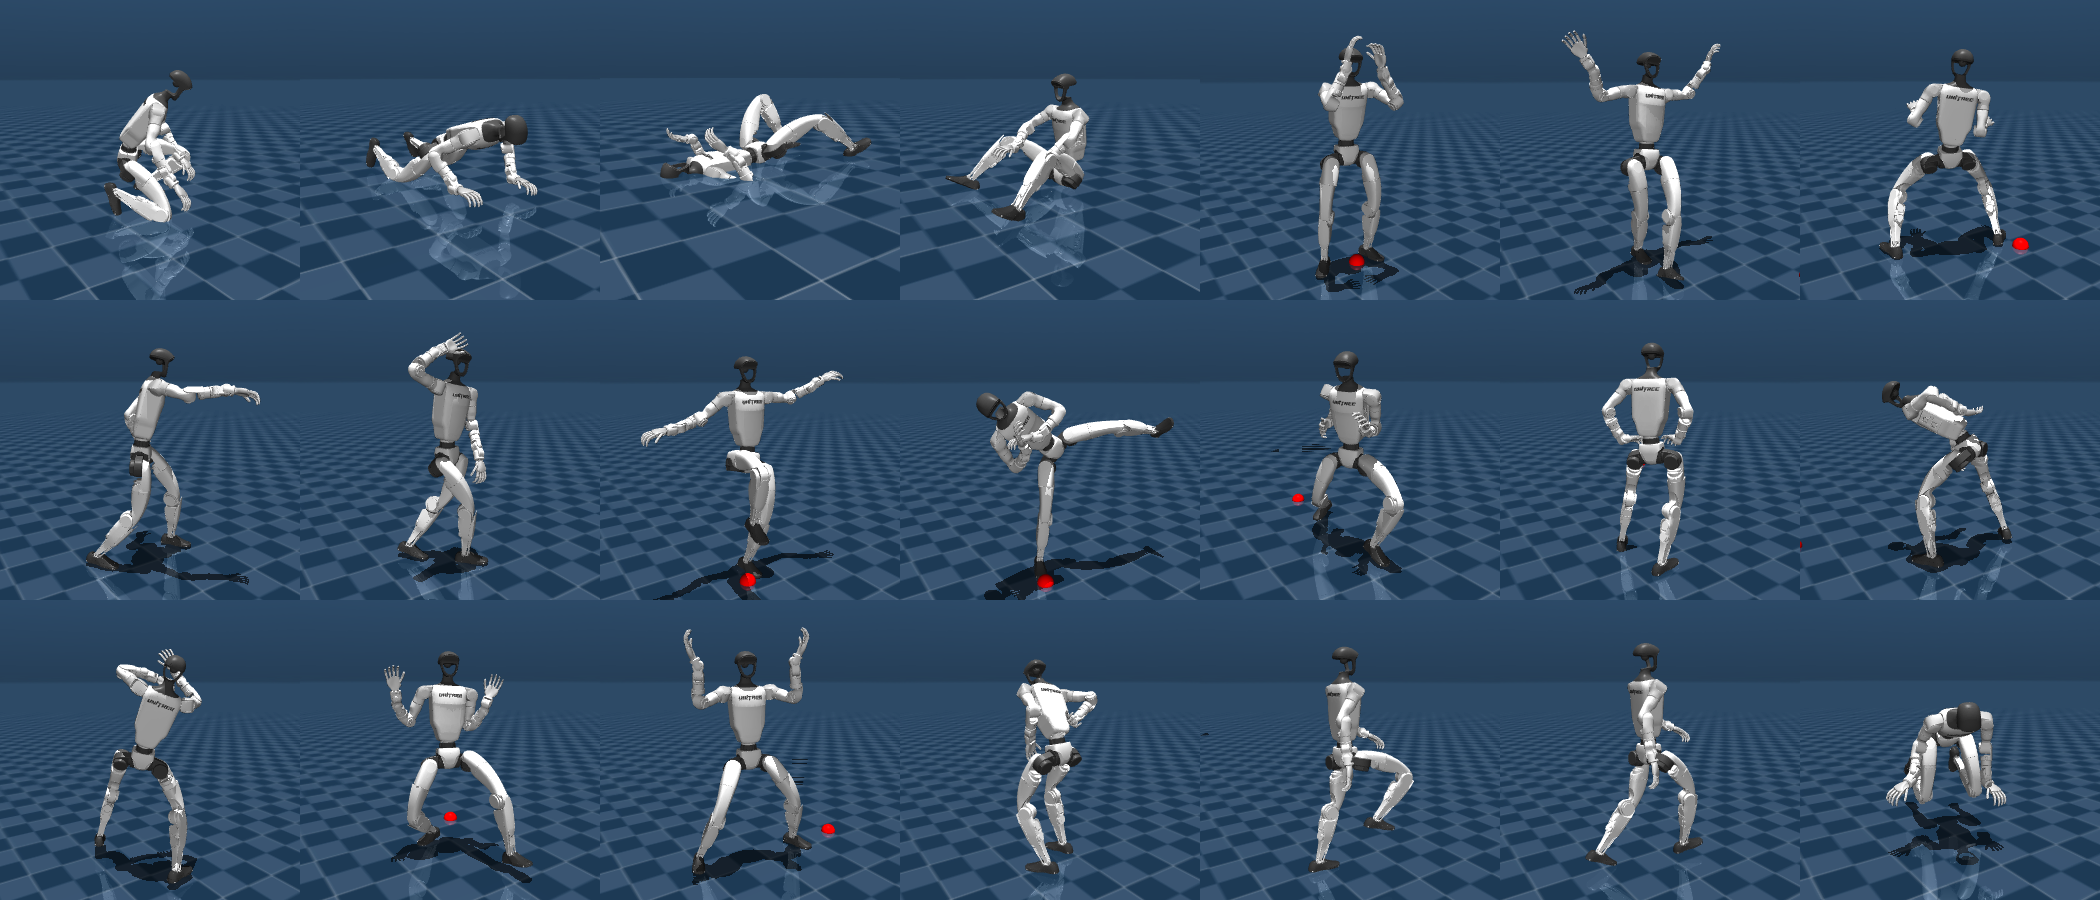
\includegraphics[width=.99\linewidth]{image/selected_goals_lafan29dof}
    \caption{Goal poses selected from frames of the LAFAN1 dataset~\citep{HarveyYNP20lafan1}.}
    \label{fig:poses_lafan}
\end{figure}

\paragraph{Tracking evaluation}
This evaluation aims to assess the ability of the model to imitate a sequence of poses, ideally matching both positions and velocities. We evaluate the agent both on the train dataset (i.e., LAFAN1) and on out-of-distribution motions selected from AMASS (retargeted to G1). In particular, we randomly selected $175$ motions from the CMU dataset of AMASS. For evaluation, we use the same metric as in goal evaluation, i.e.,
\[
E_{\mathrm{mpjpe}}(e, m) = \frac{1}{|e|}\sum_{t=1}^{|e|} \|q_t(e) - q_t(m)\|_2
\]
and we report the average across motions.

\paragraph{Reward evaluation}\label{app:rewards}
We define $6$ reward categories inspired by~\citep{TirinzoniTFGKXL25zeroshot}. The reward can be expressed as a function of the next state and normalized in $[0,1]$.

\textit{Standing}. We evaluate the agent's ability to stand with the pelvis at different heights. \texttt{move-ego-0-0} requires pelvis above 60cm and zero velocity, while \texttt{move-ego-low0.5-0-0} requires the pelvis to be between 50cm and 65cm.

\textit{Locomotion}. This category includes rewards related that requires the agent to move at a certain speed, in a certain direction and at a certain height. We consider $5$ representative rewards (\texttt{move-ego-0-0.7}, \texttt{move-ego-90-0.7}, \texttt{move-ego-(-90)-0.7}, \texttt{move-ego-0-0.3}, \texttt{move-ego-180-0.3}) which include forward, lateral and backward movement. We additionally test also walking forward but with the pelvis at a low height (\texttt{move-ego-low0.6-0-0.7}).

\textit{Rotation}. We require the robot to rotate along the vertical axis (i.e., while standing). We consider rotating clockwise and counterclockwise (i.e., \texttt{rotate-z-5-0.5} and \texttt{rotate-z-(-5)-0.5}).

\textit{Ground poses}. To further stress the ability of the model to control the vertical position, we define rewards requiring the agent to sit on the ground (\texttt{sitting}) or having the pelvis slightly above the ground (\texttt{crouch-0.25} is about 25cm above the ground).

\textit{Arm raise}. We require the robot to stand in a steady position and to reach a certain vertical position with the arms (measured at the wrists). We consider low ($z \in [0.6m, 0.8m]$) and medium ($z > 1m$) positions for the wrists, with soft margins (\texttt{raisearms-l-l}, \texttt{raisearms-l-m}, \texttt{raisearms-m-l}, \texttt{raisearms-m-m}).


\textit{Combined rewards.} We finally evaluate the ability of the agent to maximize rewards that require combining multiple skills. In particular, we test combinations of locomotion and rotation with arm movements. We selected $8$ combinations of rewards.


Overall, we tested $24$ rewards and evaluated perfomance via the cumulative
return over episodes of $T = 500$ steps. The initial state of an episode is the default pose.